\chapter{Wyznaczenie odpowiedzi skokowych oraz badanie w�a�ciwo�ci obiektu}

\section{Odpowiedzi skokowe}

W celu uzyskania odpowiedzi skokowych zosta�y przeprowadzone symulacje dla r�nych skok�w warto�ci sterowania $G1$ i $G2$ z punktu pracy. Wymaga�o to doprowadzenia obiektu do punktu pracy po czym zmiany warto�ci jedego z wej��.

\begin{figure}
	\centering
	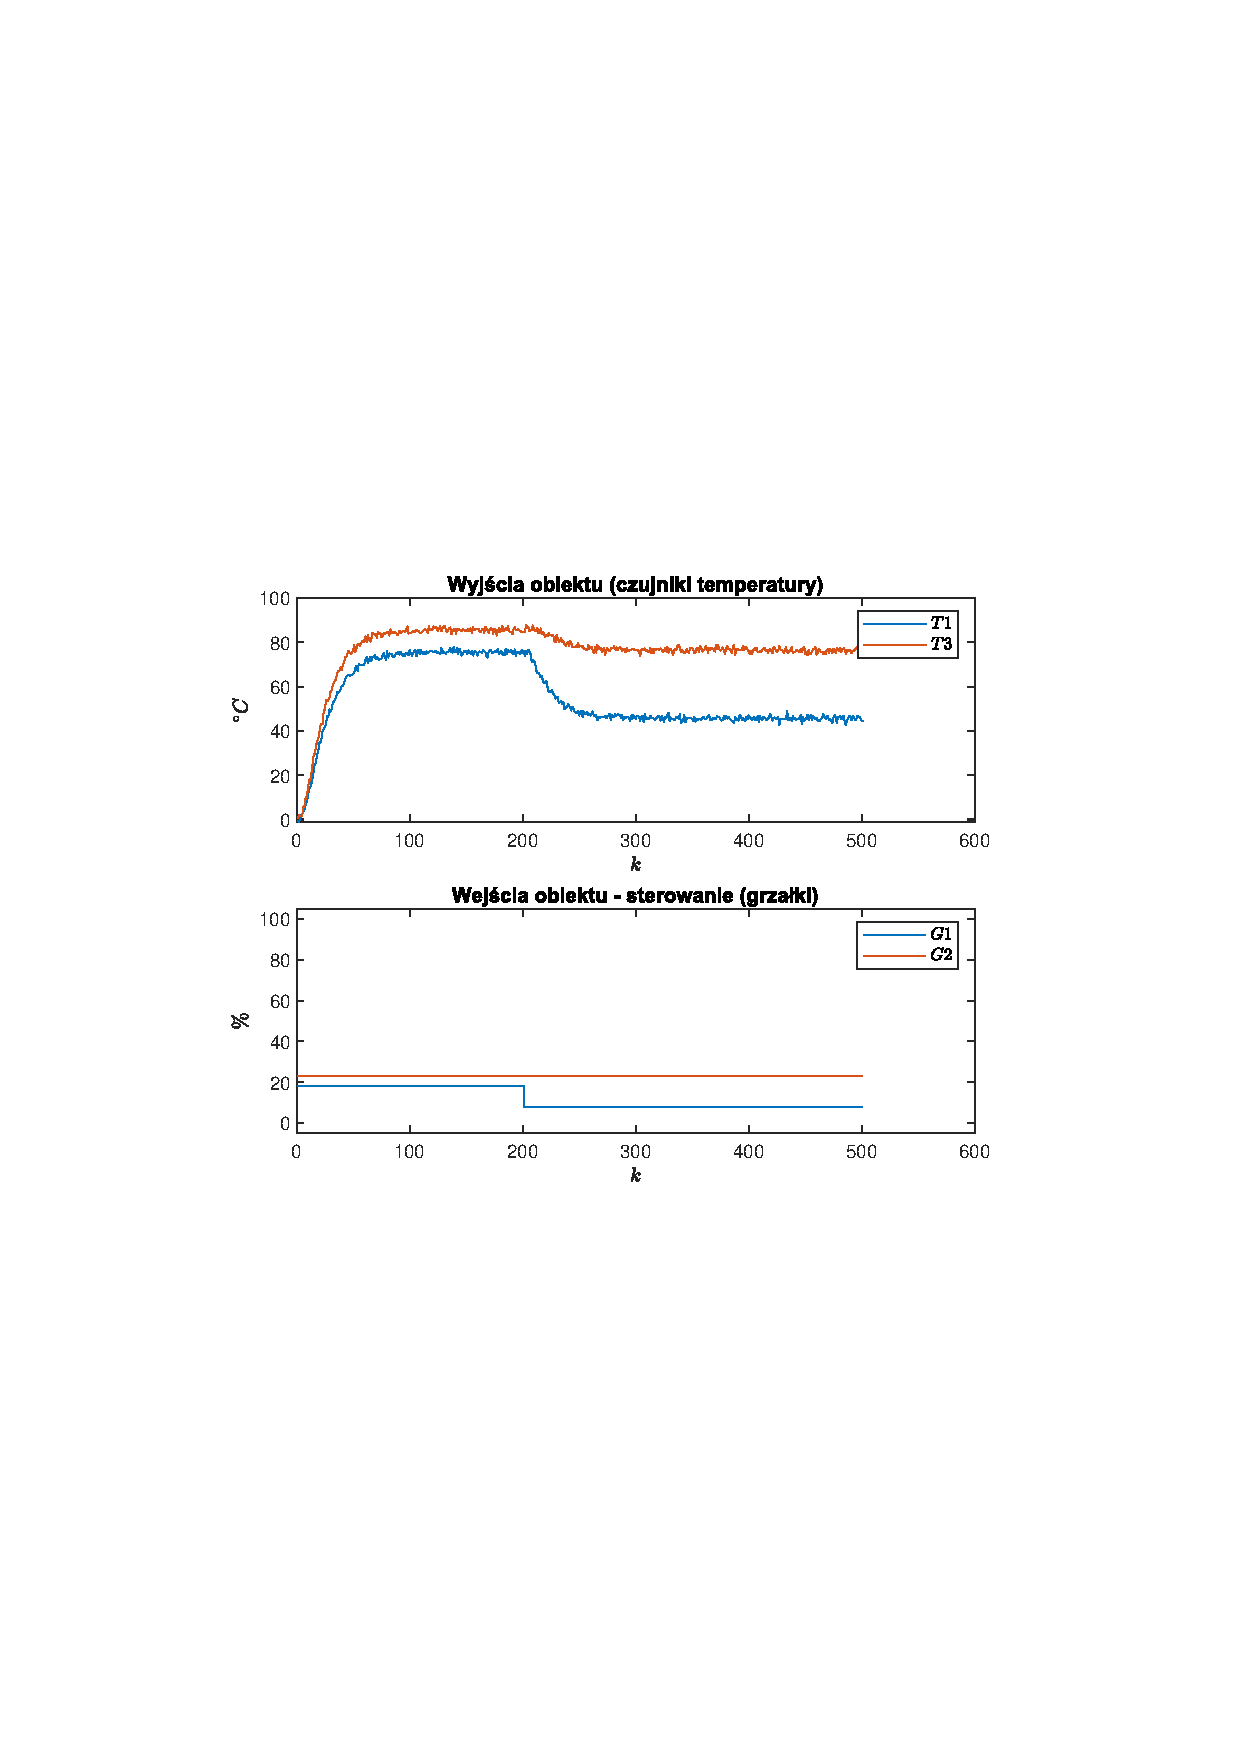
\includegraphics[scale=0.85, trim={2cm 8.5cm 2cm 8.5cm}]{rysunki/skok_g1_8_g2_23}
	\caption{Skok sygna�u sterowania $G1$ z $\num{18}$ na $\num{8}$  z punktu pracy}
	\label{skok_g1_8_g2_23}
\end{figure}

\begin{figure}
	\centering
	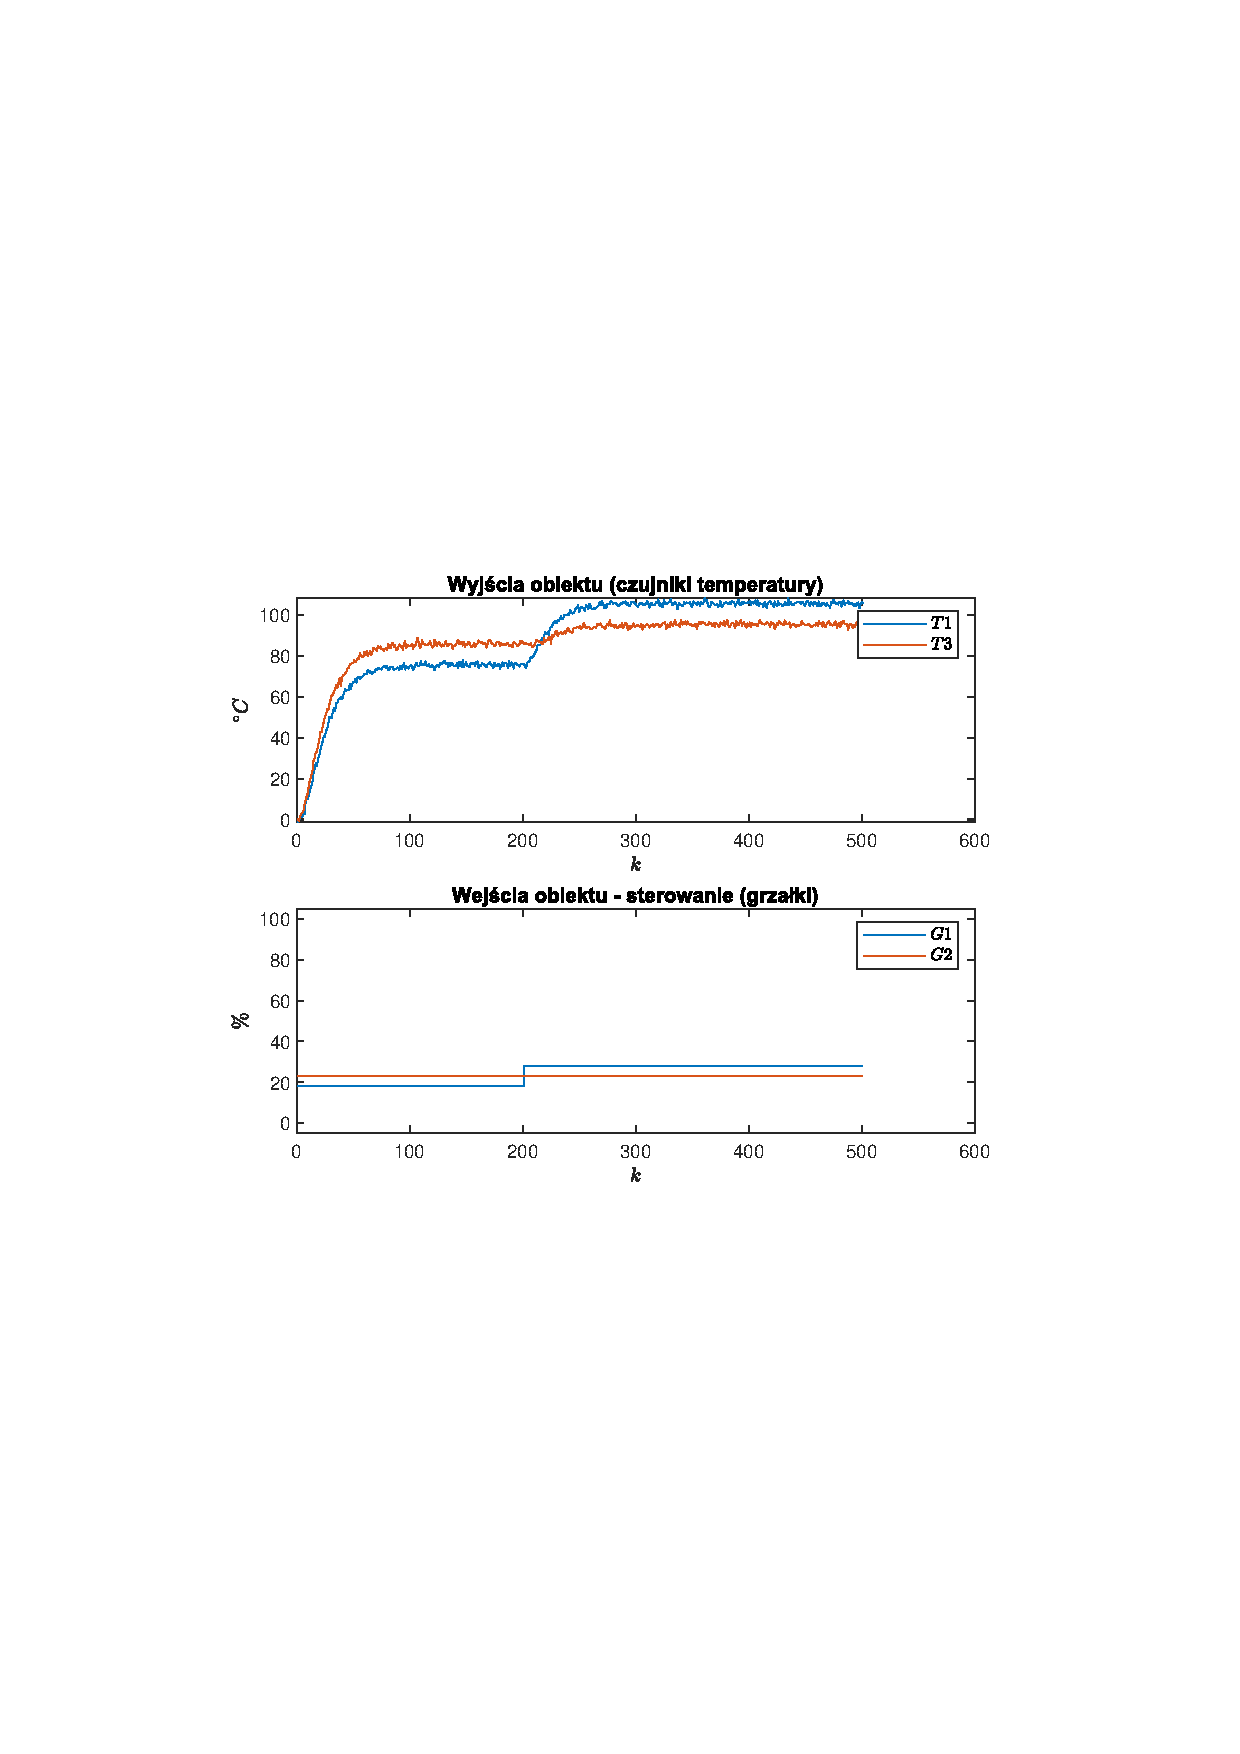
\includegraphics[scale=0.85, trim={2cm 8.5cm 2cm 8.5cm}]{rysunki/skok_g1_28_g2_23}
	\caption{Skok sygna�u sterowania $G1$ z $\num{18}$ na $\num{28}$  z punktu pracy}
	\label{skok_g1_8_g2_23}
\end{figure}

\begin{figure}
	\centering
	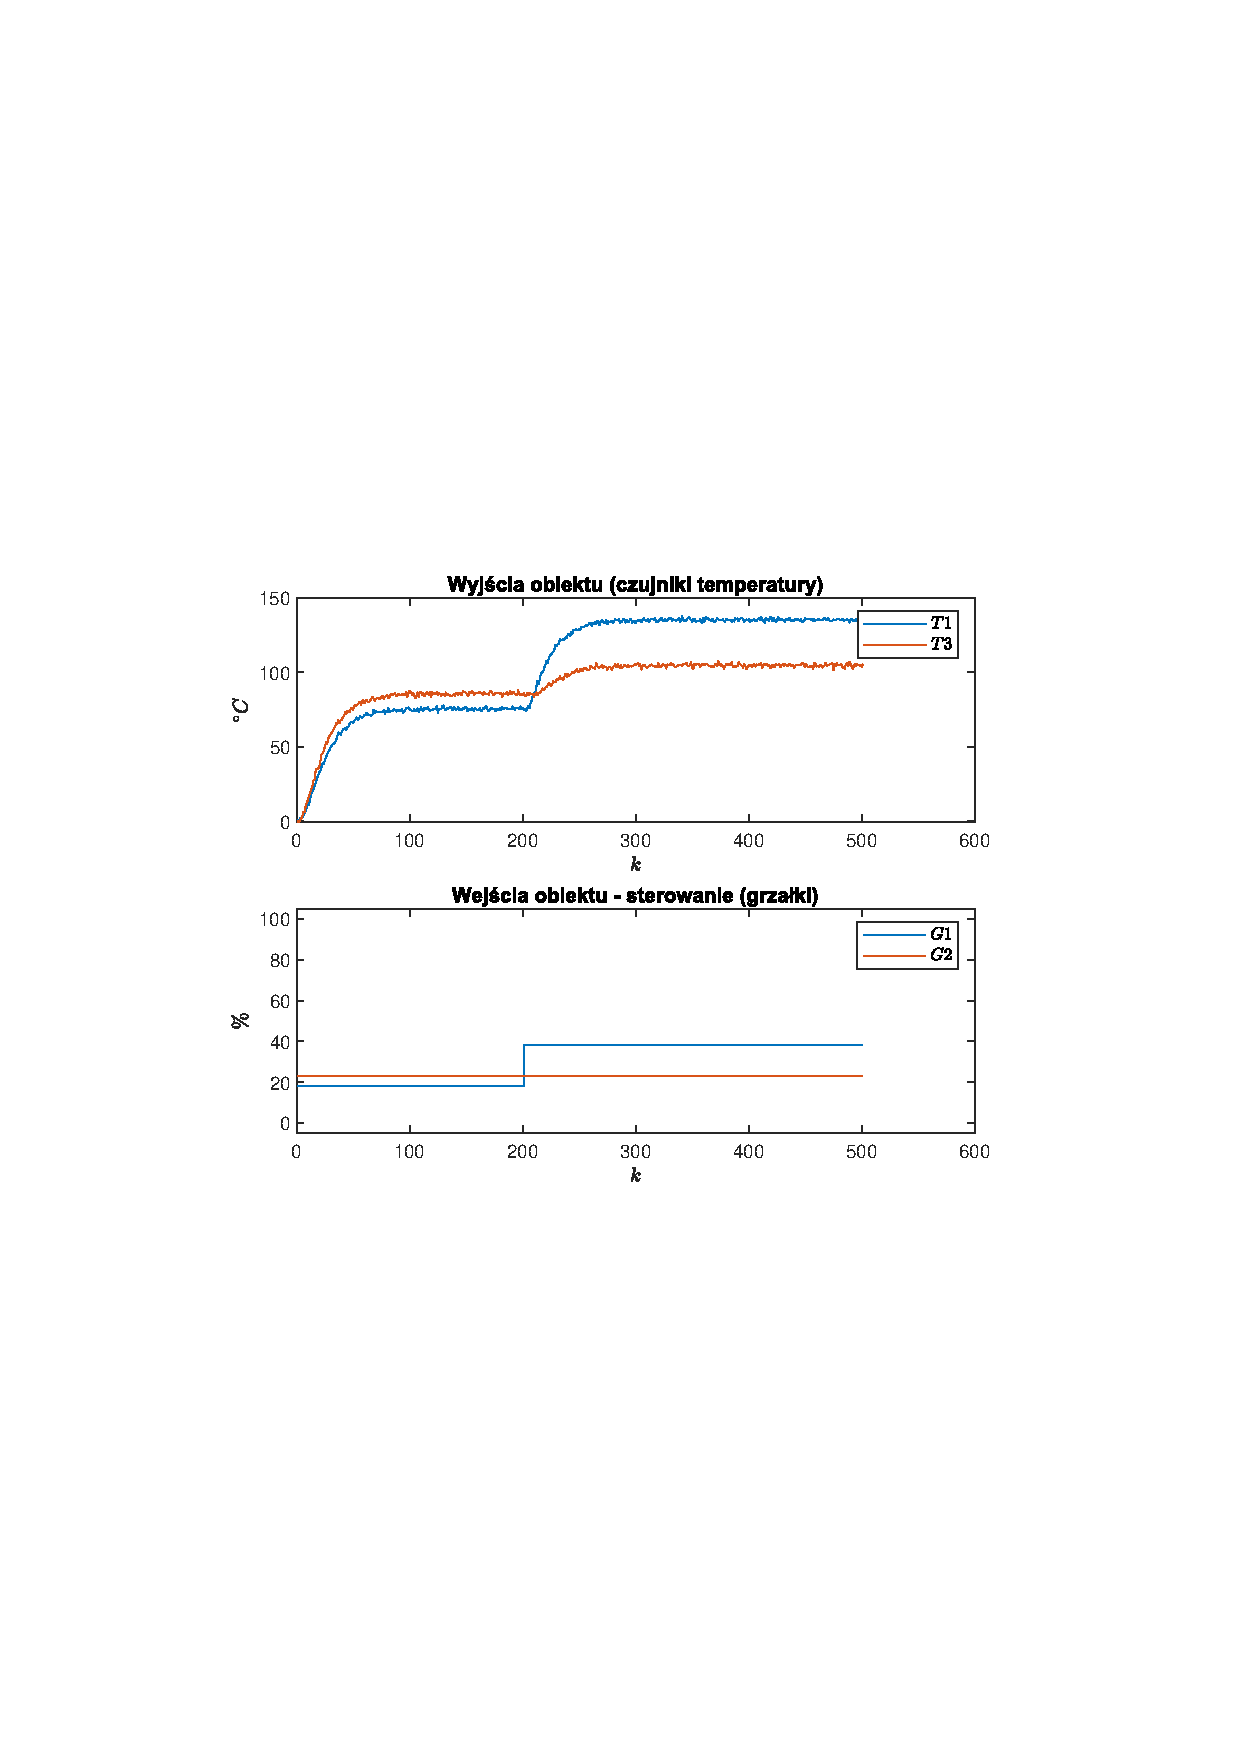
\includegraphics[scale=0.85, trim={2cm 8.5cm 2cm 8.5cm}]{rysunki/skok_g1_38_g2_23}
	\caption{Skok sygna�u sterowania $G1$ z $\num{18}$ na $\num{38}$  z punktu pracy}
	\label{skok_g1_8_g2_23}
\end{figure}

\begin{figure}
	\centering
	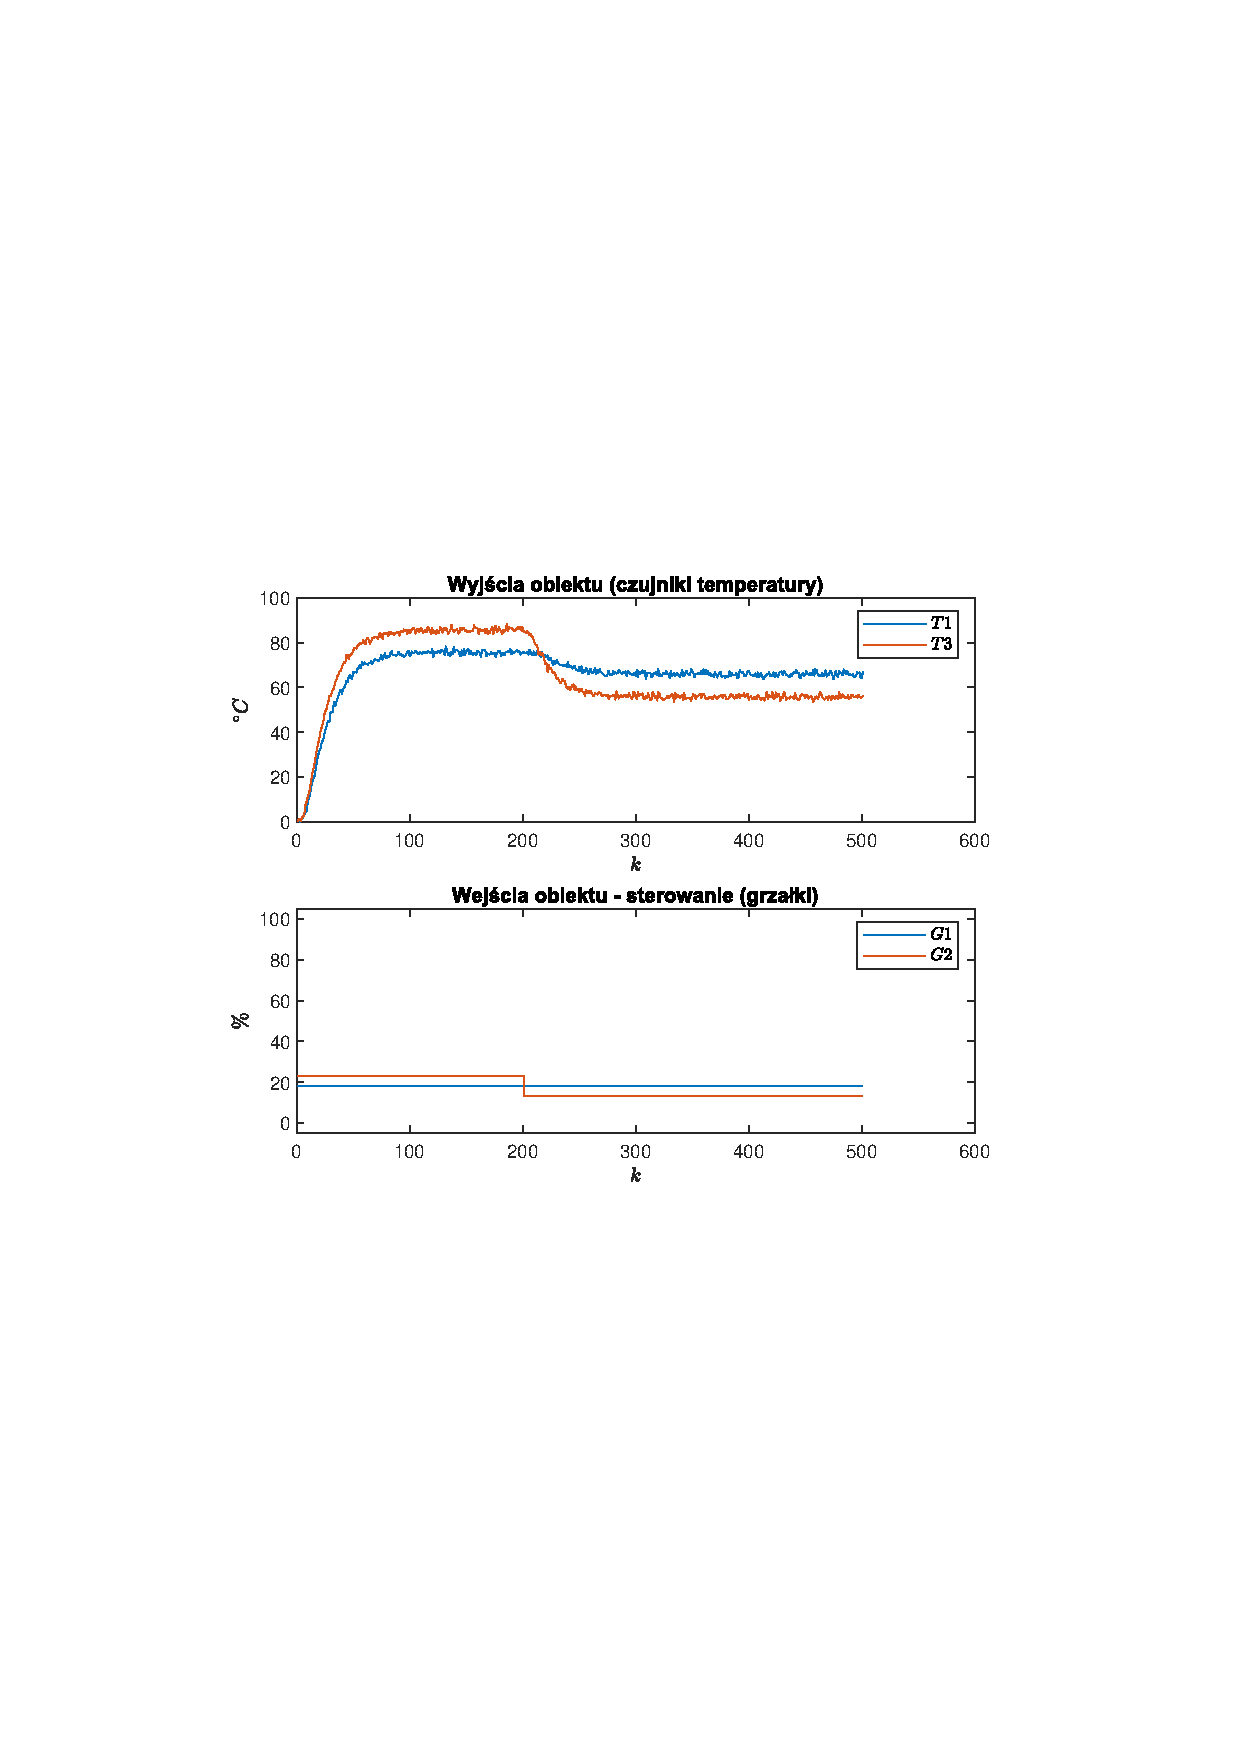
\includegraphics[scale=0.85, trim={2cm 8.5cm 2cm 8.5cm}]{rysunki/skok_g1_18_g2_13}
	\caption{Skok sygna�u sterowania $G2$ z $\num{23}$ na $\num{13}$  z punktu pracy}
	\label{skok_g1_8_g2_23}
\end{figure}

\begin{figure}
	\centering
	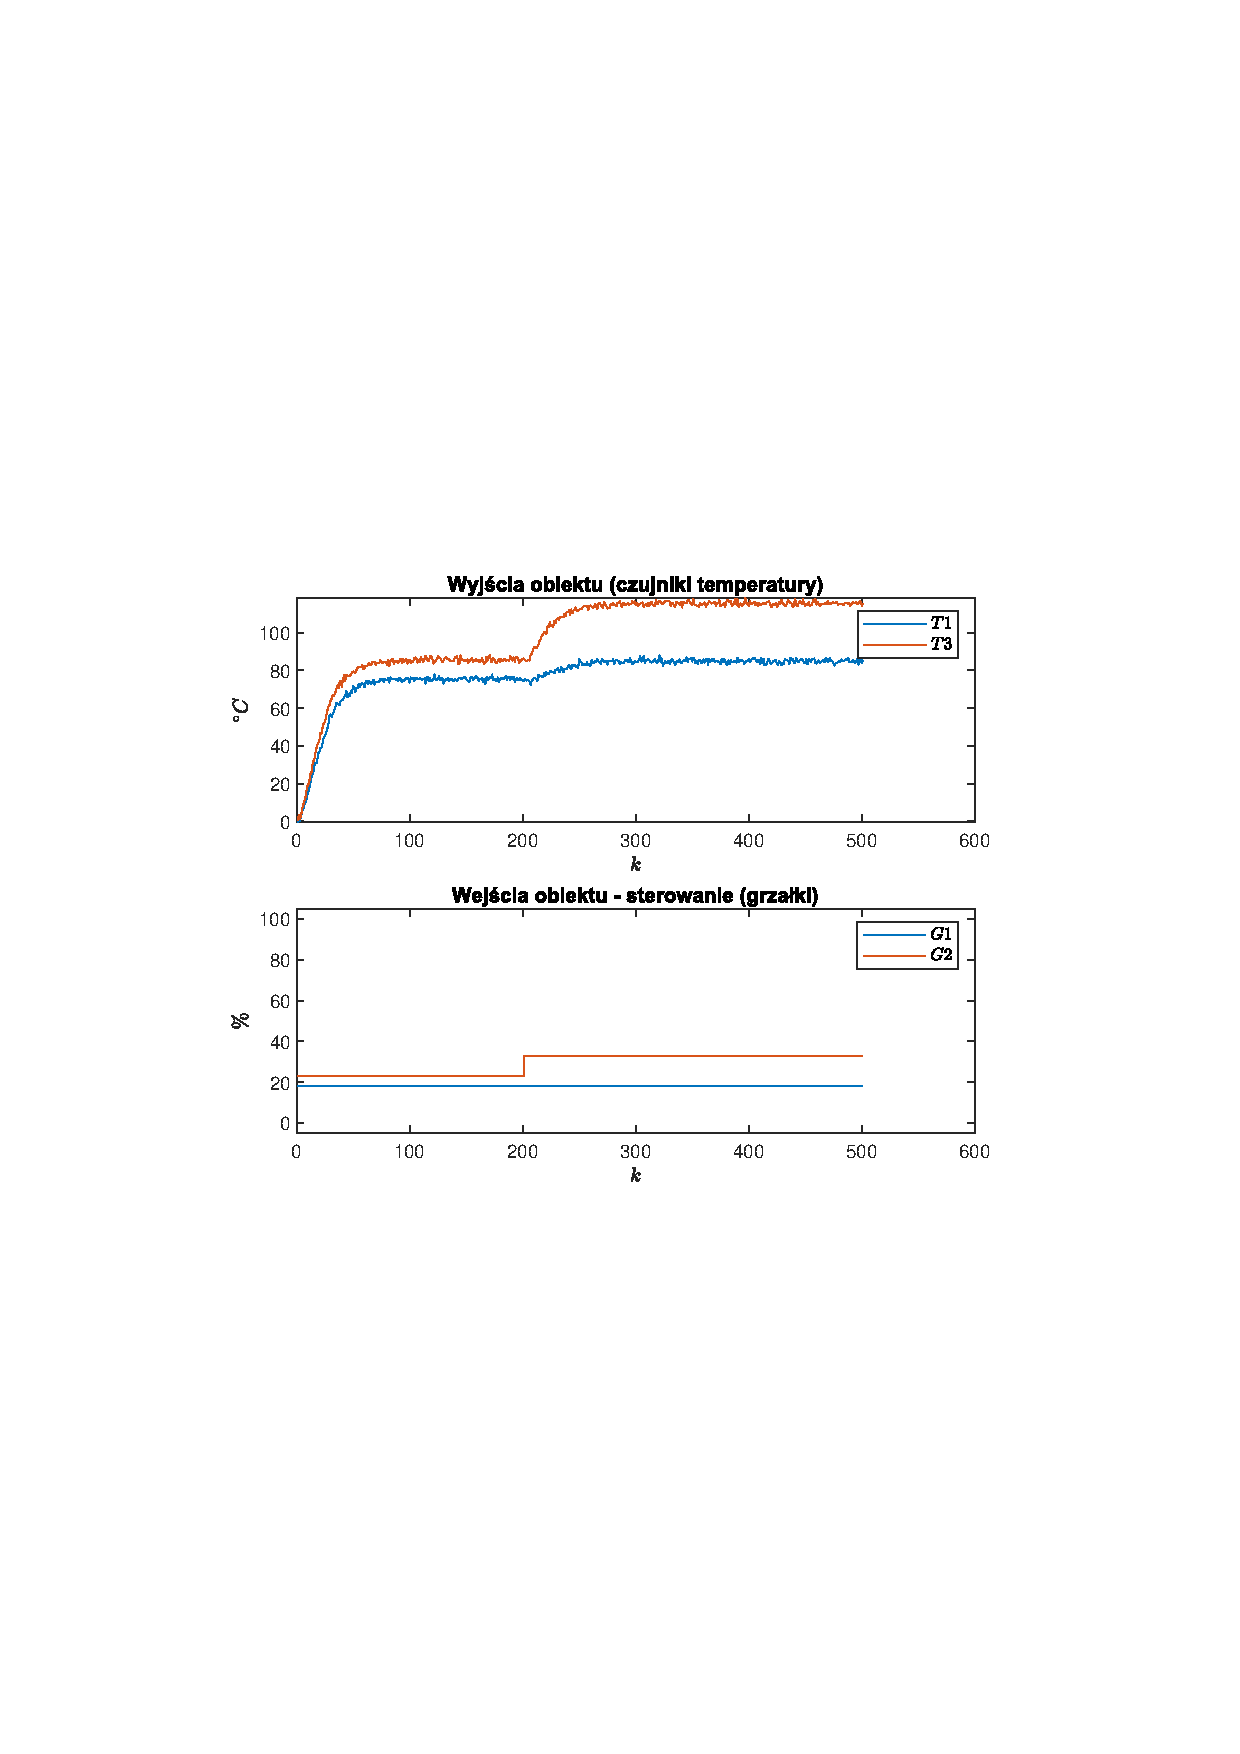
\includegraphics[scale=0.85, trim={2cm 8.5cm 2cm 8.5cm}]{rysunki/skok_g1_18_g2_33}
	\caption{Skok sygna�u sterowania $G2$ z $\num{23}$ na $\num{33}$  z punktu pracy}
	\label{skok_g1_8_g2_23}
\end{figure}

\begin{figure}
	\centering
	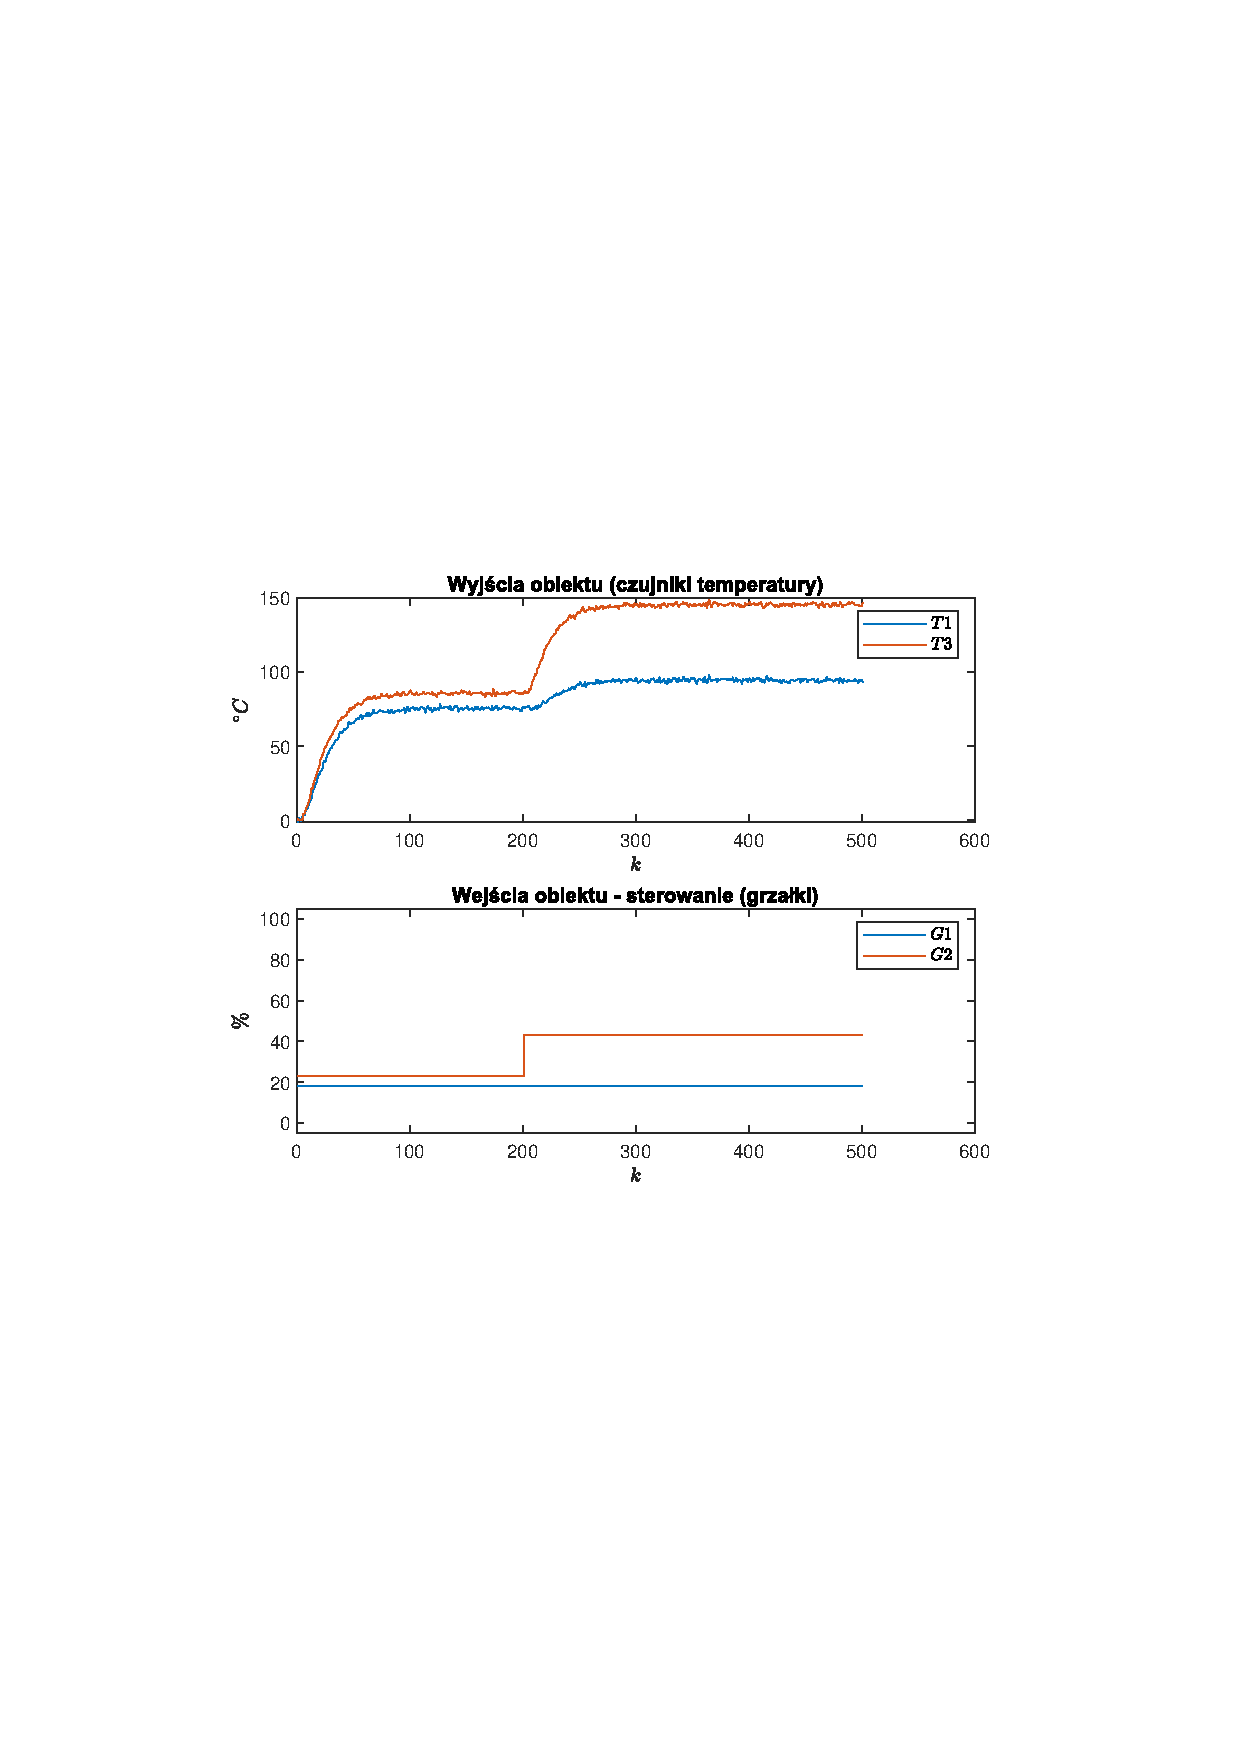
\includegraphics[scale=0.85, trim={2cm 8.5cm 2cm 8.5cm}]{rysunki/skok_g1_18_g2_43}
	\caption{Skok sygna�u sterowania $G2$ z $\num{23}$ na $\num{43}$  z punktu pracy}
	\label{skok_g1_8_g2_23}
\end{figure}

Poni�ej zosta�y przedstawione wykresy odpowiedzi skokowych dla r�nych zmian, warto�ci sterowania $G1$ i $G2$.

\begin{figure}
	\centering
	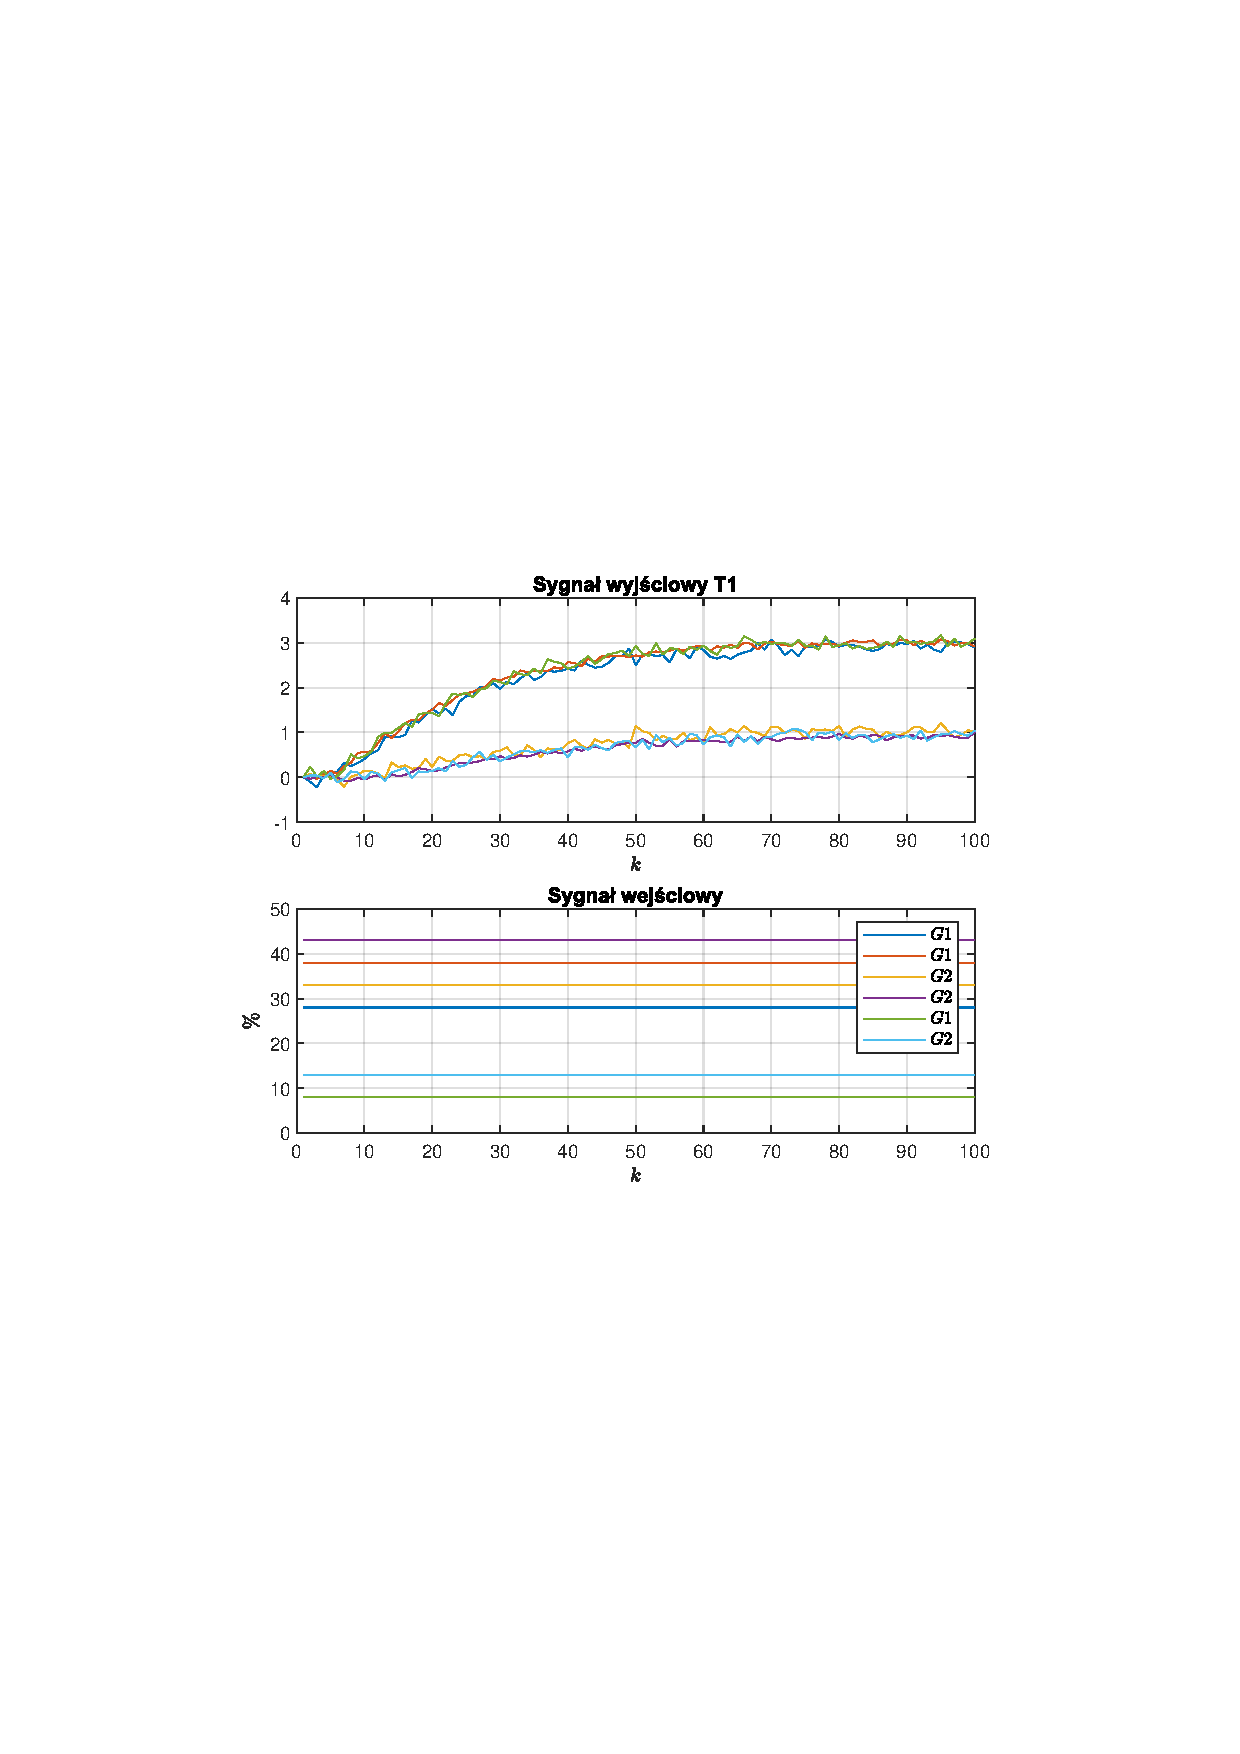
\includegraphics[scale=0.85, trim={2cm 8.5cm 2cm 8.5cm}]{rysunki/odp_skok_t1}
	\caption{Odpowied� skokowa obiektu dla wyj�cia $T1$}
	\label{odp_skok_t1}
\end{figure}

\begin{figure}
	\centering
	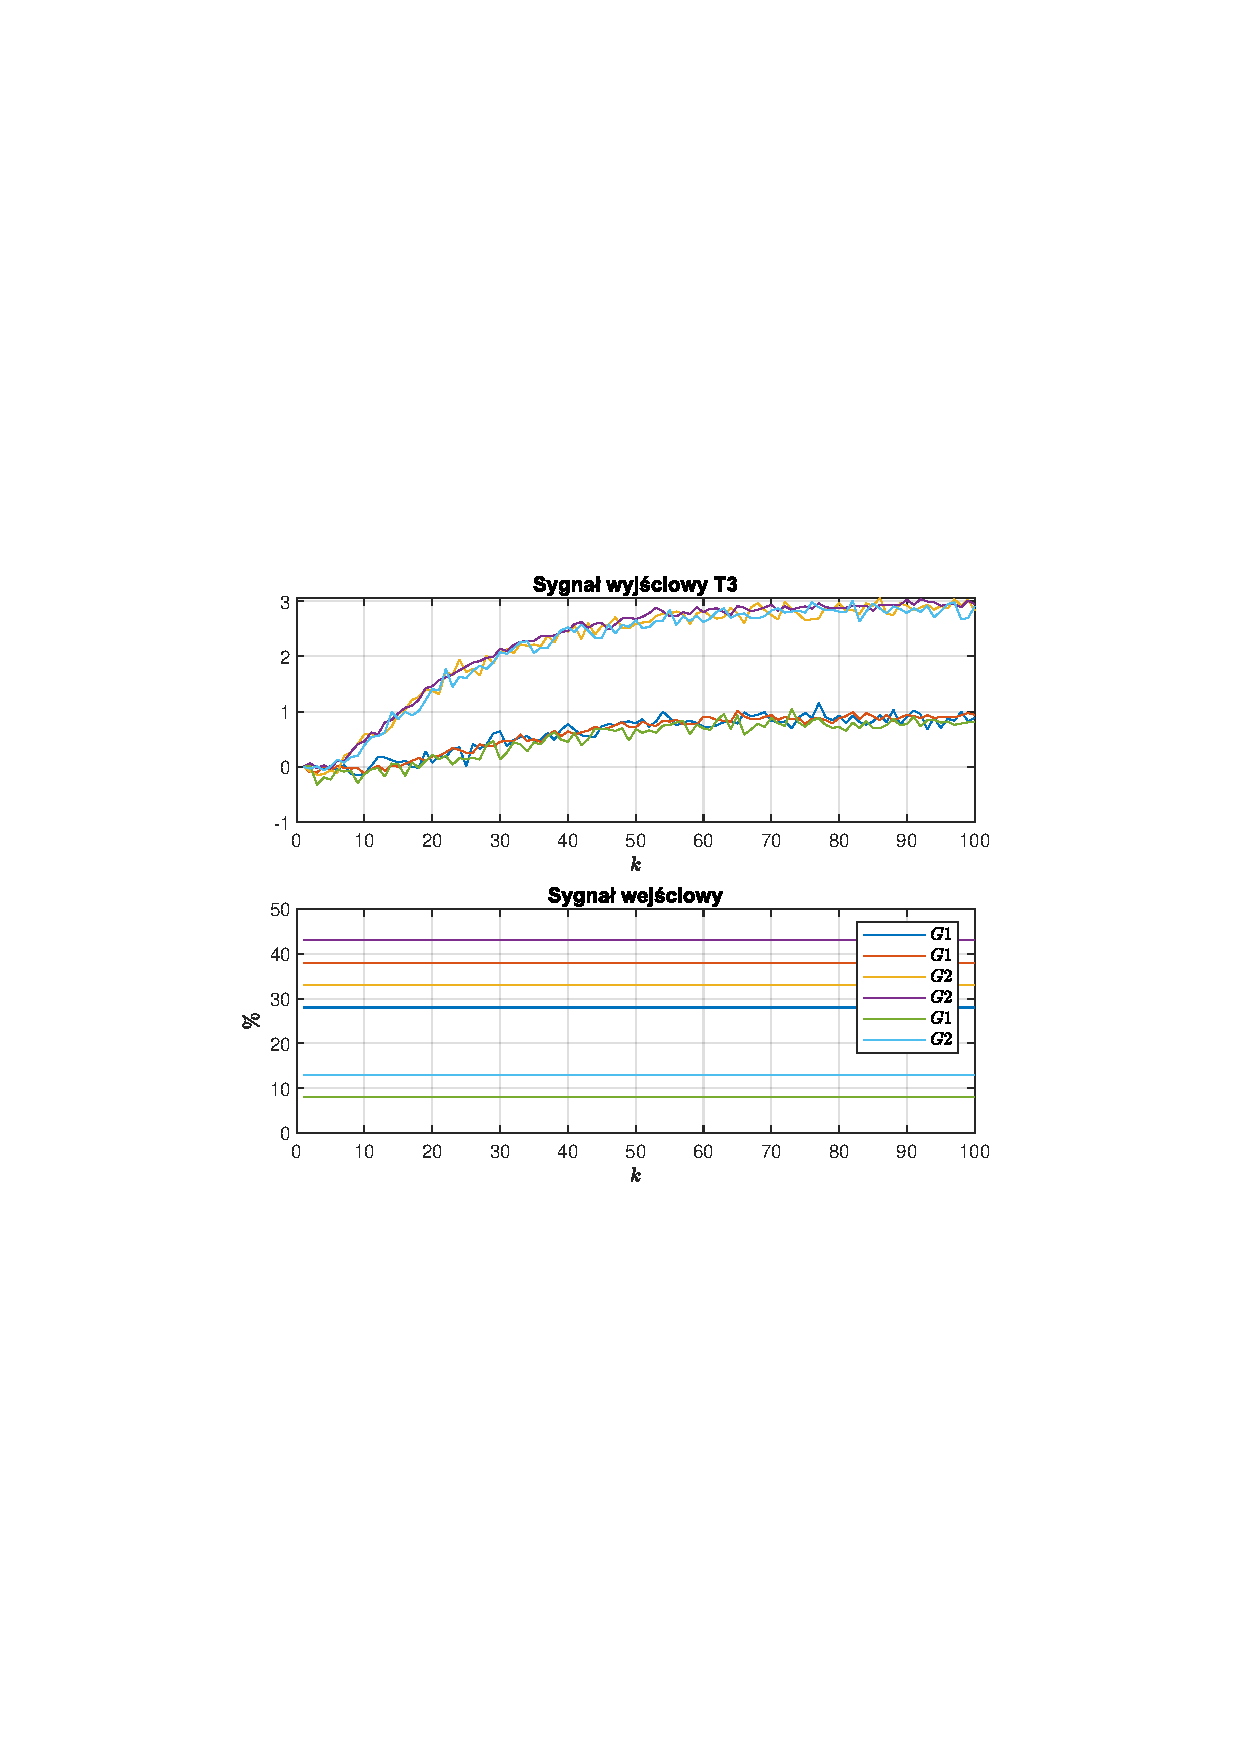
\includegraphics[scale=0.85, trim={2cm 8.5cm 2cm 8.5cm}]{rysunki/odp_skok_t3}
	\caption{Odpowied� skokowa obiektu dla wyj�cia $T3$}
	\label{odp_skok_t1}
\end{figure}



\section{W�a�ciwo�ci statyczne obiektu}

Mo�emy zauwa�y� �e w�a�ciwo�ci statyczne obiektu s� nieliniowe.